\section{Angewandte Ansätze für die Erkennung von Design Patterns}

Bei der Erkennung von Design Patterns in Quellcode wurden verschiedene Verfahren entwickelt werden, die auf unterschiedlichen Methoden beruhen, um das gesetzte Ziel zu erreichen.
Yarahmadi et al.~führten in ihrer Arbeit eine Untersuchung über die Methoden, die angewandt worden, um Design Patterns in Quellcode zu erkennen, und kategorisierten diese~\cite[S. 5805]{yarahmadi2020design}.

\begin{figure}[h]
    \centering
    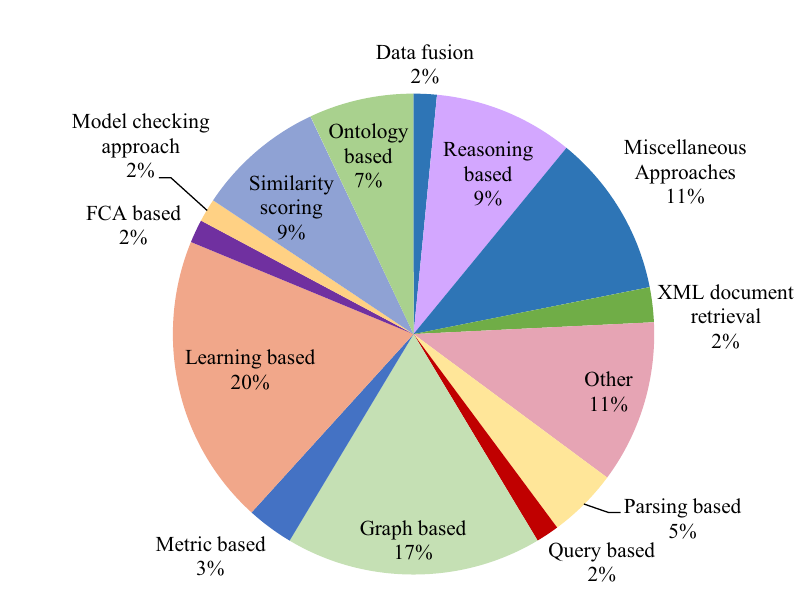
\includegraphics[scale=0.5]{figures/approches_distribution.png}
    \caption{Verteilung der Kategorien der Ansätze für die Erkennung von Design Patterns in Quellcode}
    \label{fig:approach_dist}
\end{figure}

Wie aus Figur~\ref{fig:approach_dist} zu entnehmen ist, wurden die entwickelten Prozesse von Yarahmadi et al. auf eine begrenzte Menge an Kategorien eingestuft.
In dieser Sektion der Arbeit werden die vier größten Kategorien aus Figur~\ref{fig:approach_dist} genauer erläutert und es werden exemplarisch Arbeiten diskutiert,
die in die jeweilige Kategorie zugeordnet werden können. 

\subsection{Graphen-basierende Ansätze}

Die Methodik der Reduktion stellt in der Berechenbarkeitstheorie einen Ansatz dar, um Lösungswege für neue unbekannte Probleme zu entwickeln. Dabei wird durch einen Algorithmus das unbekannte Problem in ein bereits gelöstes Problem, dessen Lösungsweg bereits vorhanden ist, umgewandelt.
In Graphen-basierenden Methoden für die Erkennung von Design Pattern in Quellcode wird diese angewendet, um Quellcode in Graphen zu transformieren und diese Graphen werden als Eingabe für diverse Graphenalgortihmen verwendet.

\pagebreak

Formell betrachtet ist ein Graph definiert als~\cite[S. 9]{Siu1998IntroductionTG}:
\begin{align*}
& \text{G} = \{V(G), E(G)\}
&\\
&\text{mit}
&\\
&G : \text{der zu betrachtende Graph}\\
&V (G): \text{Nicht leere Menge von Knoten in G}\\
&E (G): \text{Menge an ungeordneten Tupeln von distinkten Elementen von V (G)}
\end{align*}

Der Quellcode selbst ist als roher Text zu betrachten, welches verschiedene Entitäten wie Klassen, Objekte und Schnittstellen beinhaltet, und definiert, wie diese miteinander interagieren. Als Graph $G$ werden die Entitäten aus dem Quellcode als Knoten $V (G)$ und 
die Relationen und Interaktionen wie Vererbung oder Methodenaufrufe werden als Kanten $E (G)$ dargestellt.
Hierbei stellt Unified Modeling Language (UML) eine in der Software-Entwicklung verbreitete Modellierungssprache dar und definiert verschiedene Arten von Graphen dar, um Software und andere Systeme zu modellieren.
Die Diagramme aus der UML-Domäne werden in diesem Kontext als Graphen aufgefasst, da diese aus einer Menge aus Kanten und Konten bestehen und anhand der obigen Definition als Graphen interpretiert werden können.
Eine Diagrammart aus der Domäne, welches eingesetzt wird, um objektorientierte (OO) Software-Systeme zu modellieren, sind Klassendiagramme.
Klassendiagramme beschreiben, wie Klassen und deren Relation zueinander im Kontext des Paradigmas der OO-Programmierung aufgefasst werden.
Pradhan et al.\ nutzen Klassendiagramme als Eingabe für ihre entworfene Methode und generieren diese für das zu analysierende Software-System und Implementierung von Entwurfsmustern, die als Referenz genutzt werden~\cite[S. 2]{7346680}.
Diese werden als gerichtete Graphen erfasst, wobei die Klassen als Knoten und die Assoziation wie Vererbung zwischen diesen als Kanten darstellen. Zusätzlich werden die Kanten je nach Art der Assoziation unterschiedlich gewichtet~\cite[S. 2]{7346680}.
Im weiteren Verlauf werden mögliche Menge Kandidaten aus dem Graphen des Software-Systems als dessen Subgraphen durch die Eigenschaft der Graphenisomorphie extrahiert und anhand der normalisierten Kreuzrelation der Maß der Übereinstimmung bestimmt~\cite[S. 3]{7346680}.
Graphenisomorphie beschreibt, ob zwei Graphen die strukturell identisch sind, sodass jede Kante des einen Graphen einer Kante im anderen Graphen entspricht und umgekehrt~\cite[S. 10]{Siu1998IntroductionTG}. Die normalisierten Kreuzrelation ist ein Maß, dessen Wertebereich zwischen 0.0 und 1.0 definiert ist.
Je näher der Wert an 1.0, desto identischer sind die zwei Graphen. 
Zu der Evaluierung des Prozesses wurden vier Open Source Software-Systeme hergezogen, aus welchen fünf existierende Entwurfsmuster zu erkennen sind~\cite[S. 6]{7346680}. Dabei wurde von Pradhan et al. dokumentiert, ob ein Entwurfsmuster komplett oder partiell im Quellcode entdeckt wurde.
Nach eigener Auswertung von Pradhan et al. wurden die als Referenz genommen Implementierung der Design Patterns mehrfach komplett als auch partiell in der Codebasis der zu dem Test hergezogen Software-Systeme identifiziert~\cite[S. 6]{7346680}.

\pagebreak

In ihrer Arbeit verfolgen Dongjin et al. in ihrer vorgeschlagenen Methodik ebenfalls die Erkennung von Entwurfsmustern der strukturellen Kategorie in Quellcode durch den Einsatz von Graphen. In Kontext dieser werden wie im vorherigen Verfahren beschriebenen Klassendiagramme als gerichtete gewichtete Graphen eingesetzt.
Entitäten wie Klassen, Objekte oder Schnittstellen als Knoten und die Assoziation der Entitäten wie Vererbung als gerichtete gewichtete Kanten des repräsentiert~\cite[S. 582]{6649882}.
Zudem werden Referenzimplementierung der zu identifizierenden Entwurfsmuster in gewichtete Klassendiagramme transformiert und innerhalb dieser werden Submuster definiert, die in Summe das Entwurfsmuster repräsentieren~\cite[S. 580]{6649882}.

\begin{figure}[h]
    \centering
    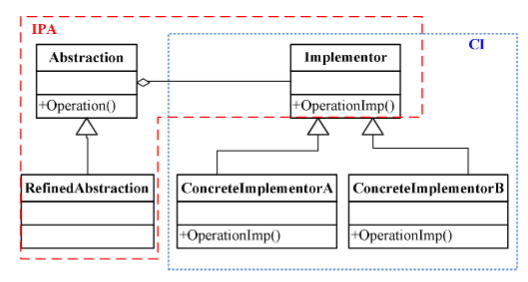
\includegraphics[scale=0.75]{figures/struture_bridge.png}
    \caption{Referenzklassendiagramm des Bridge Patterns mit Submustern}
    \label{fig:structure_bridge}
\end{figure}

Beispielhaft spiegelt die Abbildung \ref{fig:structure_bridge} von Dongjin et al. definierte Referenzklassendiagramm für das Bridge Pattern wider. Innerhalb dieses Klassendiagramms werden die Submuster \textbf{IPA} und \textbf{CI} festgelegt. Wie von der Abbildung \ref{fig:structure_bridge} zu entnehmen ist, bestehen die Submuster aus einzelnen Entitäten und deren Assoziationen.
Innerhalb der Klassendiagramme des Quellcodes, welches als Eingabe dient, wird nach solchen Submustern durch Einsatz von Graphenisomorphie gesucht~\cite[S. 584]{6649882}. Im weiteren Verlauf werden identifizierte relevante Submuster zu einer Kandidatsstruktur verschmolzen. Dabei ist anzumerken, dass nur die Submuster, die in Kontext des betrachtenden Entwurfsmusters assoziiert sind, im Vorgang der Verschmelzung involviert sind.
Als finaler Schritt in dieser Methodik werden durch Analyse des Verhaltungsmusters der Kandidatsstrukturen falsch positiv identifizierte Instanzen herausgefiltert~\cite[S. 584]{6649882}. Im Kontext dient Quellcode aus vier Open Source Software-Systemen als Eingabe für dieses Verfahren~\cite[S. 585]{6649882}. 
Zu Evaluierung der Resultate der Methodik wird die Metrik der \textit{Precision} verwendet. Dabei wird das Verhältnis zwischen der Anzahl der positiv falschen identifizierten Instanzen zu der Summe der Anzahl der positiv falsch und falsch positiv klassifizierten Instanzen gebildet~\cite[S. 585]{6649882}. Je höher diese ist, desto besser ist das Ergebnis einzustufen.
Nach eigenständiger Evaluierung von Dongjin et al. wird für alle Software-Systeme für alle betrachten strukturellen Entwurfsmuster eine hohe Rate der \textit{Precision} ermittelt~\cite[S. 586]{6649882}

%TODO: Add this file:///home/memi/Downloads/Yu,%20Dongjin_%20Zhang,%20Yanyan_%20Ge,%20Jianlin_%20Wu,%20Wei%20-%20[IEEE%202013%20IEEE%2037th%20Annual%20Computer%20Software%20and%20Applications%20Conference%20(COMPSAC)%20-%20Kyoto,%20Japan%20(2013.07.22-2013.07.26)]%20201%20(2013,%20IEEE)%20[10.1109_COMPSAC.2013.92]%20-%20libge.pdf

\pagebreak

\subsection{Maschine Learning Ansätze}

Mit der ersten öffentlich zugänglichen Version des Open Source Maschine Learning Frameworks TensorFlow am 9. November 2015, wurde der Zugang für praktisch angewandtes Maschine Learning
für Software-Entwickler erleichtert. Durch TensorFlow wird eine Abstraktionsschicht für das Entwerfen, Trainieren und den Betrieb von Machine Learning Modellen, vor allem neuronalen Netzwerken, vereinfacht
und somit die Anwendung von Maschine Learning in Produkten und in der Forschung populärer. Dieses ist auch der Fall für die Erkennung von Design Patterns in Quellcode.
Wie aus Abbildung~\ref{fig:approach_dist} zu entnehmen, stellen nach der Untersuchung von Yarahmadi et al. Verfahren, die Maschine Learning einsetzen, einen signifikanten Teil dar.
Im Kontext dieser Aussage werden in diesem Abschnitt ausgewählte Verfahren erläutert, die Maschine Learning als Teil des Erkennungsprozesses involvieren.

%%TODO: Start with this Research on Design Pattern Detection Method Based on UML Model with Extended Image Information and Deep Learning


\subsection{Similarity-Scoring Ansätze}

\subsection{Diverse Ansätze}



